\chapter{基于RBF-SVR的分片逼近模型在直复营销下广告预算分配中的研究}

% 首先介绍多渠道广告投放资金分配问题使用强化学习研究的现状(没有利用强化学习解决该问题的文献,存在的主要问题:数据量较少,导致值函数估计不准确等问题,收敛速度慢,说明本文采用非参数化建模的原因,非参数化建模又存在什么问题,针对此问题又是如何解决的)
% 介绍深度强化学习
% 介绍本文提出的混合网络模型算法
% “我知道我的广告费有一半浪费了,可是我不知道浪费的是哪一半。”美国费城商人约翰·华纳梅克的这句自嘲式的调侃简直让人抓狂——似乎你绞尽脑汁想出的营销点子就是为了达到一个目的——尽量让广告费被浪费得少一点而已。

\section{直复营销下广告预算分配问题阐述}
在本部分中,首先介绍了在直复营销体系下,借助第三方广告代理商进行广告投放的应用背景及其具体的投放过程。然后,说明了广告投放的目标是追求全渠道的LTV最大化,以此来解释选择强化学习解决该问题的原因。最后,介绍了广告投放场景所具有的三个特点,并考虑针对这些特点来优化强化学习算法,将此作为本章研究的出发点。

\subsection{广告预算分配场景}
美国直复营销协会(American Direct Marketing Association,ADMA)\footnote{http://www.the-dma.org/}将直复营销(Direct Response Marketing)定义为一种市场营销体系,运用一种或几种广告媒介在任何地点产生可以度量的反应或交易。直效营销仅仅属于直复营销中的一种应用场景,它特指不通过第三方,中间人,而直接对客户进行推广和营销,以维持企业与客户的良好关系。但是,在这种场景下需要企业有充足的客户资源和大量的相关客户资料,这对于大部分企业是很难办到的,需要很长时间的积累,特别是在日益激烈的市场竞争环境中,时间就是企业的生命线。于是,为了快速获取用户、推广相关产品、扩大公司的收入,越来越多的企业选择通过第三方广告代理商(Ad-agency)进行广告投放。

广告代理商除了帮助企业进行广告设计与策划以外,还有一部分更重要的工作,就是帮助广告主安排或代为购买媒介空间或时间。近年来,随着广告市场的不断发展和扩大,为了方便广告主高效的进行广告投放,大部分在线的广告代理商也都建设了自己的广告投放平台,其投放流程如图$\ref{fig:lstm_2}$所示。在广告投放平台上,广告代理商(Ad-agency)有很多可供选择的广告渠道(channel)资源,广告主每次需要提供一个广告投放策略,策略的内容包括在哪些渠道上投放广告以及对应投放多少金额的广告费。然后,广告代理商会按照广告主提供的投放策略,将对应的广告量通过各渠道投放给潜在顾客(广告的受众)。在广告投放结束后,广告代理商会将此次广告投放的直观效果反馈给广告主,同时广告主也可以通过追踪已经交易的顾客的后续信息,综合评价此次的投放效果。

\begin{figure}[htbp]
\centering
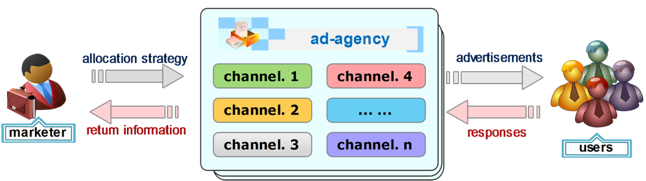
\includegraphics[width=0.8\textwidth]{ad_process}
\caption{基于ad-agence的广告投放过程}
\label{fig:ad_process}
\end{figure}

通过以上的介绍,可以看到在通过广告代理商投放广告的过程中,顾客可以及时接收到广告主发布的广告信息,而广告主也会收到响应顾客的响应反馈,因此广告主与顾客之间是存在互动性的。另外,广告主还可以根据广告代理商反馈的投放效果信息以及追踪用户未来行为等方式去量化此次广告投放对企业的价值,因此效果是可衡量性的,所以,利用广告代理进行广告投放的方式也属于直复营销体系。

在企业进行广告投放的真实业务中,为了保证财务帐面的稳定以及公司合理健康的发展,公司财务每个月都会给出该月的广告投放资金的预算,然后广告投放部门会在此预算下进行广告预算的合理分配,以使得公司的业务不断扩大、收入持续增长。但是,因为广告投放场景比较复杂,单纯靠广告投放人员制定预算分配策略往往很持续难达到好的效果,所以需要充分利用机器学习技术。

\subsection{生命周期价值}
通常情况下,企业在进行广告投放时,为了达到持久有效的营销效果,而且为了能够更好的评价广告渠道的质量,一般都会在一个广告代理商下进行为期一年或几年的持续投放。因此,广告投放是一个序列化的过程。

另外,在进行广告投放的过程中,存在效果延迟的问题。比如一个顾客在某一时刻看到该广告,但是并没有立刻产生正向反馈或者交易,而是在经过若干时间后的某一时刻才有正向反馈。那么,此时所产生的收益不单单与现在这个时刻的广告投放效果有关,还与之前的广告投放效果有关。因此,在评价广告投放的效果时,不能单单考虑该条广告的即时收益。所以,在实际应用中,广告主一般将广告渠道的LTV作为评价广告质量的重要指标。通过第二章的介绍,我们知道强化学习在处理序列问题时,很好的考虑到了延迟奖赏的问题,并且以追求累积奖赏最大化作为优化目标,所以将强化学习技术应用在广告投放领域,可以充分发挥其优势。

\subsection{广告预算分配特点}
% 多渠道/总预算限制/数据量少
然而,在广告投放过程还存在诸多问题,如果直接应用强化学习,无法取得很好的效果。

首先,对于大部分企业来说,广告投放是以天为单位进行的,所以投放数据量比较少,这样会严重影响模型的训练。因此,为了提高数据的使用率,我们考虑使用非参数化函数的逼近方法进行强化学习的训练。另外,一般在广告投放时会选择多个渠道同时进行投放,所以,我们不单单要考虑到渠道自身的延迟反馈,而且还应该考虑渠道间的相互影响。最后,每一次的广告投放策略都是在一个给定的预算下制定的,即我们在每次在作出投放策略时都会受一个固定预算的约束,所以我们在得到Q值后结合多选择背包问题进行最终预算分配策略的定制。所以,我们在应用强化学习技术的时候要综合考虑这些问题,作出响应的改进。

\section{基于RBF-SVR的分片逼近模型}
\subsection{分片思想}
\subsection{RBF-SVR模型}

\section{强化学习在多渠道广告投放预算分配中的建模设计}
\subsection{花费空间离散化方法}
\subsection{渠道间投放影响}
\subsection{改进的探索方法}
\subsection{MCKP结合方法}
\subsection{整体架构}